\documentclass{article}
\usepackage{graphicx}
\usepackage{geometry}
\geometry{a4paper, margin=1in}

\title{Wing Optimization Report}
\date{2025-06-04}

\begin{document}
\maketitle

\section{Executive Summary}
This report summarizes the optimization process performed to minimize the drag coefficient (CD) of a wing, subject to a lift coefficient (CL) constraint of 2.0, a wing area of 100 m$^2$, and a span of 10 m. The design variables included taper, twist, and sweep. The optimization was conducted using the SLSQP optimizer. While the optimization reduced the drag, it ended with a 'FAIL' status, indicating non-convergence. The final drag coefficient achieved was approximately 0.1184.

\section{Problem Formulation}
The optimization problem was formulated as follows:
\begin{itemize}
    \item Objective Function: Minimize drag (CD)
    \item Trim Condition: CL = 2.0
    \item Geometric Constraint: Wing area (S) = 100 m$^2$, Span (b) = 10 m
    \item Design Variables: Taper, Twist, Sweep
    \item Optimization Algorithm: SLSQP
\end{itemize}

\section{Optimization Results}
The optimization process ran for 18 iterations and terminated with a 'FAIL' status, suggesting that the solution did not fully converge within the specified tolerance and maximum iteration limit. The final drag coefficient (CD) achieved was approximately 0.1184. The figure \ref{fig:OptimizedWing} shows the optimized visualization of the wing.

\begin{figure}[h!]
    \centering
    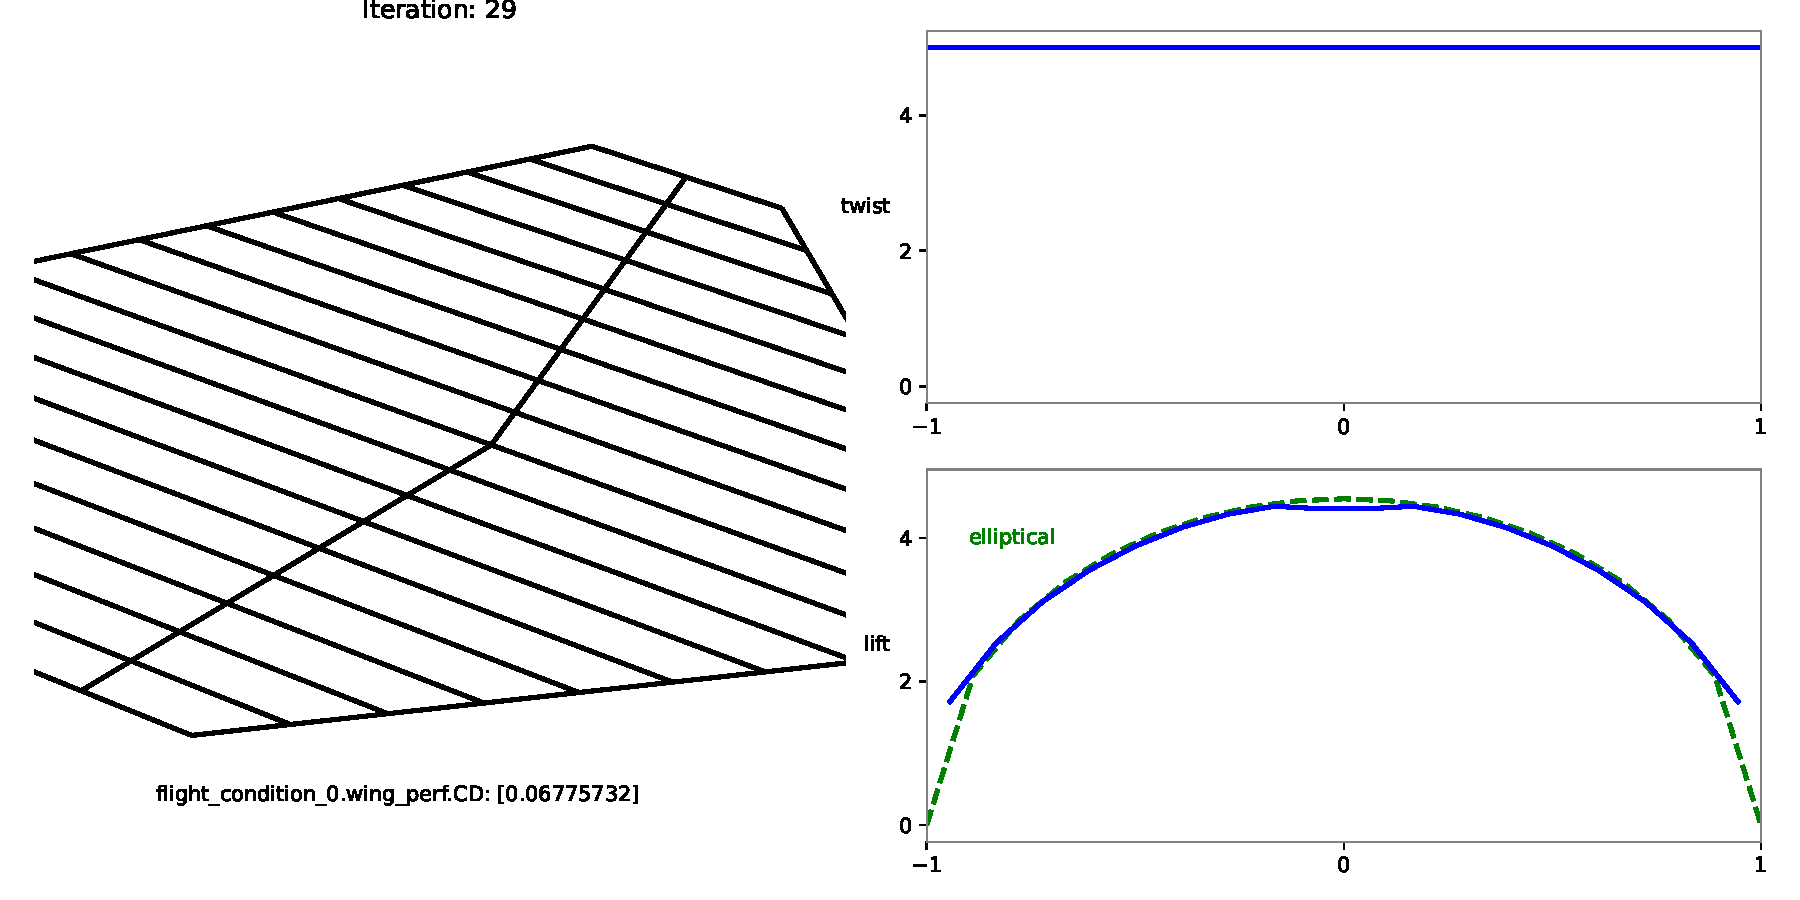
\includegraphics[width=0.75\textwidth]{./Optimized_Wing.pdf}
    \caption{Optimized Visualization of the Wing}
    \label{fig:OptimizedWing}
\end{figure}

\section{Analysis and Recommendations}
\subsection{Convergence Issues}
The 'FAIL' status indicates that the optimization did not fully converge. This could be due to several factors, including insufficient iterations or a tolerance level that is too strict. 

\subsection{Recommendations}
\begin{enumerate}
    	\item \textbf{Increase Maximum Iterations:} Increase the `maxiter` parameter in the optimizer settings to allow the optimization to reach a more optimal solution.
    	\item \textbf{Adjust Tolerance:} Experiment with the `tol` parameter. A smaller tolerance may lead to a more accurate solution, but it will also require more iterations and computational time.
    	\item \textbf{Consider Gradient-Based Methods:} For problems with many design variables, gradient-based methods may be more efficient. Gradient free methods such as genetic algorithms or particle swarm optimizers should also be considered.
    \item \textbf{Refine Design Variable Bounds:} The design variables hit the upper and lower bounds, so they should be made wider to see if a better optimum is possible.
    \item \textbf{Mesh Refinement:} Since OpenAeroStruct uses VLM, ensure the mesh resolution is adequate. Increase the number of chordwise and spanwise panels to capture the flow accurately, especially twist. The lift distribution should also be checked with a higher fidelity solver.
\end{enumerate}

\subsection{Optimization Performance}
The optimization was performed using the SLSQP optimizer, which is a gradient-based method. While SLSQP is generally efficient, alternative optimizers such as genetic algorithms or particle swarm optimization might be beneficial for more complex problems or those with many local minima.  

\subsection{Unrelated Observations}
It is important to note that the OpenAeroStruct code assumes that the wing is symmetric. To gain further confidence in the solution, a higher fidelity code should be used to validate the results. Additionally, the optimizer uses SLSQP, which is a local optimizer, meaning that the solution obtained is only locally optimal. Factors such as manufacturability and structural integrity should also be considered during the design process, as these may impose additional constraints or influence the selection of design variables.

\section{Concluding Remarks}
Further investigation and refinement of the optimization settings are recommended to achieve full convergence and explore potentially better solutions. Validation with higher-fidelity codes and consideration of real-world constraints are essential for a practical wing design.


\end{document}